\subsection{线性判别分析（LDA）}
\label{sec:classification-lda}

用花瓣长度与宽度区分两类鸢尾花时，只比较两类平均长度可能会遗漏宽度提供的信息。把两项测量相加也未必合适：如果某项测量在同类花之间就有很大波动，它对区分类别的作用可能不及另一项；两项测量相关时，还要考虑它们是否重复提供了同一份信息。我们需要据此确定各特征的权重，并选择划分类别的阈值。

一种办法是先描述每类测量值围绕中心怎样变化，再比较新样本来自各类的可能性。\term{线性判别分析}（linear discriminant analysis, LDA）在高斯生成模型下采用这条路线：类均值给出中心，共享协方差刻画类内尺度与相关性，类先验记录类别比例。由这些量计算的后验概率，最终给出一个线性判别函数。协方差相同是这里的建模假设，并非所有分类数据都具有的性质。

LDA还有一个几何起点。Fisher在1936年的鸢尾花分类研究中寻找一种线性组合，使两类均值的差异相对于类内波动尽可能大。这一准则不要求样本服从高斯分布；它与高斯生成模型可以给出相同的判别方向，但概率解释和适用条件有所不同\scite{fisher1936}。

从两类的线性组合转向多个总体的判别，问题不再只是选择一条轴，还包括需要保留多少个方向。Rao在1948年系统讨论了多总体的生物分类与判别表示，这也为理解LDA如何从分类规则延伸为有监督降维方法提供了历史背景\scite{rao1948}。

\subsubsection{模型结构}
\label{sec:classification-lda-model}

沿用训练集$D_n=\{(\bm{x}_i,y_i)\}_{i=1}^{n}$，其中$\bm{x}_i\in\mathbb{R}^{d}$、$y_i\in\{1,\ldots,C\}$。生成式LDA假设
\begin{equation}
  \label{eq:classification-lda-distribution}
  \begin{aligned}
    \mathbb{P}(y=c)&=\pi_c,\qquad \pi_c>0,\quad
      \sum_{c=1}^{C}\pi_c=1,\\
    p(\bm{x}\mid y=c)&=\mathcal{N}(\bm{x};\bm{\mu}_c,\bm{\Sigma}),
      \qquad \bm{\Sigma}\succ0 .
  \end{aligned}
\end{equation}
这里$\bm{\mu}_c\in\mathbb{R}^{d}$描述第$c$类的中心，$\bm{\Sigma}\in\mathbb{R}^{d\times d}$描述类内各方向的波动及特征之间的相关性。共享协方差允许各类具有不同中心，同时规定中心附近相同的椭球形状和朝向；协方差中的非对角元仍可表示特征相关性。

在零一损失下，应选择后验概率最大的类别。取对数并展开高斯密度，有
\begin{equation}
  \label{eq:classification-lda-score}
  \begin{aligned}
    \log\{\pi_c p(\bm{x}\mid y=c)\}
      &=a(\bm{x})+\delta_c(\bm{x}),\\
    \delta_c(\bm{x})
      &=\bm{x}^{\top}\bm{\Sigma}^{-1}\bm{\mu}_c\\
      &\quad-\frac12\bm{\mu}_c^{\top}\bm{\Sigma}^{-1}\bm{\mu}_c
        +\log\pi_c .
  \end{aligned}
\end{equation}
其中$a(\bm{x})$收集了$-\bm{x}^{\top}\bm{\Sigma}^{-1}\bm{x}/2$、对数行列式和高斯归一化常数，均与类别无关。正是共享协方差使二次项在类别比较时抵消，留下关于$\bm{x}$的仿射函数。任意两类得分相等的位置通常为超平面；多分类的各类别区域由这些两两比较共同确定。

训练后把估计参数代入$\delta_c$，得到$\hat{\delta}_c$。预测规则及相应的模型后验为
\begin{equation}
  \label{eq:classification-lda-prediction}
  \begin{aligned}
    \hat f_{\mathrm{LDA}}(\bm{x})
      &=\argmax_{c\in\{1,\ldots,C\}}\hat{\delta}_c(\bm{x}),\\
    \hat p_c(\bm{x})
      &=\frac{\exp\{\hat{\delta}_c(\bm{x})\}}
        {\sum_{j=1}^{C}\exp\{\hat{\delta}_j(\bm{x})\}} .
  \end{aligned}
\end{equation}
本节对$\argmax$的平局统一选择索引最小的类别。共享协方差也限定了LDA能利用的类别差异。例如，设两类中心都在原点，一类的测量值集中在中心附近，另一类的测量值分散得更开。此时“离中心有多远”包含类别信息，但LDA中两类相同的均值使与输入有关的得分项完全相消，分类只能依据先验比例。若两类先验还相等，按真实均值形成的这组得分处处平局，固定类别的预测错误率为$1/2$。这说明该参数选择丢掉了尺度信息；整个LDA候选空间的限制将在表达能力分析中讨论。

让每类使用自己的$\bm{\Sigma}_c$，就能把这种尺度差异保留下来。这得到\term{二次判别分析}（quadratic discriminant analysis, QDA），即允许二次决策边界的高斯分类器\scite{hastie2009}。例如两类协方差分别为不同倍数的单位矩阵时，后验比较包含到原点的距离平方，可以形成围绕中心的球形边界。QDA同时需要为每类估计协方差；每类样本较少时，新增的参数也可能使估计更不稳定。

\subsubsection{参数学习}
\label{sec:classification-lda-learning}

\paragraph{生成模型的最大似然估计}
有标签样本已经给出了每个观测所属的高斯分量，因此这里不需要推断类别归属。令$n_c=\sum_{i=1}^{n}\mathbb{1}\{y_i=c\}$，暂设各类都有样本。忽略与参数无关的常数，对数似然为
\begin{equation}
  \label{eq:classification-lda-likelihood}
  \begin{aligned}
    \ell
      &=\sum_{c=1}^{C}n_c\log\pi_c
        -\frac n2\log\det\bm{\Sigma}\\
      &\quad-\frac12\sum_{c=1}^{C}\sum_{i:y_i=c}
        (\bm{x}_i-\bm{\mu}_c)^{\top}
        \bm{\Sigma}^{-1}(\bm{x}_i-\bm{\mu}_c).
  \end{aligned}
\end{equation}
对先验加入约束$\sum_c\pi_c=1$，拉格朗日驻点给出$n_c/\pi_c$为同一常数；归一化后该常数为$n$。对$\bm{\mu}_c$求导，则有$\bm{\Sigma}^{-1}\sum_{i:y_i=c}(\bm{x}_i-\bm{\mu}_c)=\bm{0}$。由此得到
\begin{equation}
  \label{eq:classification-lda-mean-prior}
  \hat\pi_c=\frac{n_c}{n},\qquad
  \hat{\bm{\mu}}_c=\frac1{n_c}\sum_{i:y_i=c}\bm{x}_i .
\end{equation}
这两个估计分别是类别出现频率和该类的样本均值。

把均值代回似然，定义\term{类内散度矩阵}（within-class scatter matrix）
\begin{equation}
  \label{eq:classification-lda-within}
  \bm{S}_{\mathrm{W}}
    =\sum_{c=1}^{C}\sum_{i:y_i=c}
      (\bm{x}_i-\hat{\bm{\mu}}_c)
      (\bm{x}_i-\hat{\bm{\mu}}_c)^{\top}.
\end{equation}
它累加每个样本相对于本类中心的偏离。用精度矩阵$\bm{\Omega}=\bm{\Sigma}^{-1}$改写剩余目标，得到$n\log\det\bm{\Omega}/2-\operatorname{tr}(\bm{\Omega}\bm{S}_{\mathrm{W}})/2$。其驻点满足$n\bm{\Omega}^{-1}=\bm{S}_{\mathrm{W}}$，故当$\bm{S}_{\mathrm{W}}\succ0$时，
\begin{equation}
  \label{eq:classification-lda-covariance}
  \hat{\bm{\Sigma}}=\frac1n\bm{S}_{\mathrm{W}} .
\end{equation}
对$\bm{\Omega}$的目标是严格凹的，因此该驻点给出最大似然解。

式~\eqref{eq:classification-lda-covariance}的分母是$n$，不是$n-C$。这种合并各类类内变动的估计称为\term{合并协方差}（pooled covariance），其无偏形式为
\[
  \hat{\bm{\Sigma}}_{\mathrm{U}}
    =\frac{\bm{S}_{\mathrm{W}}}{n-C},\qquad n>C .
\]
在共享协方差假设下，给定各类样本数，有$\mathbb{E}[\bm{S}_{\mathrm{W}}\mid y_1,\ldots,y_n]=(n-C)\bm{\Sigma}$，因为估计每个类中心各消耗一个自由度。最大似然与无偏估计是不同准则；两种估计渐近相同，但有限样本下有所区别。特别是先验不等时，整体缩放协方差会改变几何得分相对于$\log\hat\pi_c$的权重，预测边界未必相同。

闭式估计把训练归结为统计量累计和线性代数运算。稠密数据的类内散度累计需要$O(nd^2)$运算，矩阵分解需要$O(d^3)$运算。实现时分解一次$\hat{\bm{\Sigma}}$，再解$C$个线性方程组$\hat{\bm{\Sigma}}\bm{a}_c=\hat{\bm{\mu}}_c$；预存$\bm{a}_c$与常数项后，每个样本的预测成本为$O(Cd)$。这些计算要求协方差可逆。$\bm{S}_{\mathrm{W}}$奇异时，正定参数域内的最大似然解不存在，需用降维或正则化重新规定估计问题。

\paragraph{Fisher投影的学习}
生成模型之外，还可以直接比较投影后的类间分离与类内波动。令总样本均值$\hat{\bm{\mu}}=\sum_c(n_c/n)\hat{\bm{\mu}}_c$，定义\term{类间散度矩阵}（between-class scatter matrix）
\[
  \bm{S}_{\mathrm{B}}
    =\sum_{c=1}^{C}n_c
      (\hat{\bm{\mu}}_c-\hat{\bm{\mu}})
      (\hat{\bm{\mu}}_c-\hat{\bm{\mu}})^{\top}.
\]
它衡量各类中心相对于总中心的分散程度。投影到方向$\bm{w}$后，两种散度分别变为$\bm{w}^{\top}\bm{S}_{\mathrm{B}}\bm{w}$和$\bm{w}^{\top}\bm{S}_{\mathrm{W}}\bm{w}$。\term{Fisher判别准则}（Fisher discriminant criterion）取两者之比。以下假设$\bm{S}_{\mathrm{W}}\succ0$，使每个非零方向的分母都为正：
\begin{equation}
  \label{eq:classification-fisher-criterion}
  J(\bm{w})
    =\frac{\bm{w}^{\top}\bm{S}_{\mathrm{B}}\bm{w}}
      {\bm{w}^{\top}\bm{S}_{\mathrm{W}}\bm{w}},
    \qquad \bm{w}\ne\bm{0}.
\end{equation}
分子鼓励类中心远离，分母抑制同类样本投影后过于分散。

图~\ref{fig:classification-lda-projection}固定同一组二维教学样本，只改变单位投影方向。两类中心分别为$(-1,0)^{\top}$与$(1,0)^{\top}$，每类都加上偏移$(-0.3,-1)^{\top}$、$(-0.1,1)^{\top}$、$(0.1,1)^{\top}$、$(0.3,-1)^{\top}$。由这些点算得$\bm{S}_{\mathrm{W}}=\operatorname{diag}(2/5,8)$与$\bm{S}_{\mathrm{B}}=\operatorname{diag}(8,0)$，最优方向由$\bm{S}_{\mathrm{W}}^{-1}(\hat{\bm\mu}_2-\hat{\bm\mu}_1)$归一化得到$\bm w^\ast=(1,0)^{\top}$。它使投影均值相差$2$，合并类内方差为$0.05$；比较方向$\bm w_{\mathrm B}=(3/5,4/5)^{\top}$的均值间距为$1.2$、类内方差为$0.658$，所以两者的$J$分别为$20$与$180/329$。这里方差按总样本量$8$归一化；右侧浅色条只是样本投影的最小至最大范围，不能把它当作Fisher准则中的平方偏差。

\begin{figure}[htbp]
  \centering
  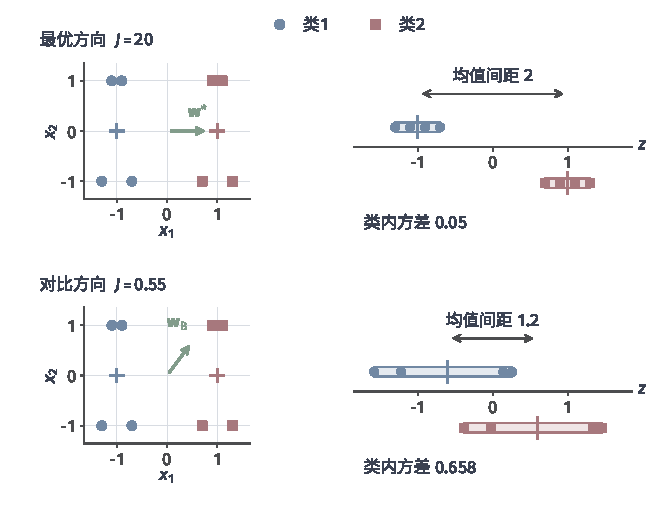
\includegraphics[width=112.000mm]{figures/04-classic-models/00-shared/matplotlib/classification-lda-target/figure.pdf}
  \caption{Fisher投影同时比较均值间距与类内散布。每类4个教学点，坐标无量纲；两行复用同一点集和相同投影数轴尺度。左侧绿色箭头为单位投影方向，十字为类均值；右侧短竖线为投影均值，浅色条为各类的样本投影范围，双向箭头标出均值间距。标注方差由$n^{-1}\bm w^{\top}\bm S_{\mathrm W}\bm w$计算，$J$仍按散度比计算。}
  \label{fig:classification-lda-projection}
\end{figure}

由于$J$不受$\bm{w}$的非零倍数缩放影响，可以约束$\bm{w}^{\top}\bm{S}_{\mathrm{W}}\bm{w}=1$。对$\bm{w}^{\top}\bm{S}_{\mathrm{B}}\bm{w}-\lambda(\bm{w}^{\top}\bm{S}_{\mathrm{W}}\bm{w}-1)$求导，得到\term{广义特征值问题}（generalized eigenvalue problem）：
\begin{equation}
  \label{eq:classification-fisher-eigenproblem}
  \bm{S}_{\mathrm{B}}\bm{w}
    =\lambda\bm{S}_{\mathrm{W}}\bm{w}.
\end{equation}
驻点还需比较大小。令$\bm{v}=\bm{S}_{\mathrm{W}}^{1/2}\bm{w}$，则
\[
  J(\bm{w})=\frac{\bm{v}^{\top}\bm{A}\bm{v}}{\bm{v}^{\top}\bm{v}},
  \qquad
  \bm{A}=\bm{S}_{\mathrm{W}}^{-1/2}
    \bm{S}_{\mathrm{B}}\bm{S}_{\mathrm{W}}^{-1/2}.
\]
把$\bm{v}$展开到对称半正定矩阵$\bm{A}$的正交特征向量上，上式就是各特征值的加权平均，权重非负且总和为$1$。最大值因而是最大特征值；取对应特征向量，再乘$\bm{S}_{\mathrm{W}}^{-1/2}$，便得到最优Fisher方向。若最大特征值有重数，最优方向未必唯一。

二分类时，令$\bm{h}=\hat{\bm{\mu}}_1-\hat{\bm{\mu}}_2\ne\bm{0}$，由总均值的定义可得
\[
  \bm{S}_{\mathrm{B}}=\frac{n_1n_2}{n}\bm{h}\bm{h}^{\top},
  \qquad
  \bm{w}_{\mathrm{F}}\propto\bm{S}_{\mathrm{W}}^{-1}\bm{h}.
\]
生成式LDA的法向量则为$\bm{w}_{\mathrm{G}}=\hat{\bm{\Sigma}}^{-1}\bm{h}=n\bm{S}_{\mathrm{W}}^{-1}\bm{h}$，两者方向相同。但完整的生成式分类规则还比较
\begin{equation}
  \label{eq:classification-lda-binary-threshold}
  \hat\delta_1(\bm{x})-\hat\delta_2(\bm{x})
    =\bm{w}_{\mathrm{G}}^{\top}
      \left(\bm{x}-\frac{\hat{\bm{\mu}}_1+\hat{\bm{\mu}}_2}{2}\right)
      +\log\frac{\hat\pi_1}{\hat\pi_2}
\end{equation}
的正负。Fisher准则本身只给方向，不给类先验、后验概率或这一阈值。两类均值相同时，均值散度准则没有正特征值方向，而生成模型仍可按先验选择类别。因此Fisher投影可用于非高斯数据，而贝叶斯最优性的证明还需要正确指定的高斯生成模型。

\subsubsection{理论分析}
\label{sec:classification-lda-analysis}

\paragraph{表达能力}
若真实类条件分布满足式\eqref{eq:classification-lda-distribution}，其后验概率就属于LDA的候选概率函数集，相应的贝叶斯决策也属于候选分类规则，无须用近似模型代替。共享协方差允许相关特征和不同类中心，但规定各类只有一个高斯峰，且峰周围的形状相同。即使不把得分解释为高斯后验，两个仿射得分的比较也只能产生一个半空间，不能表达任意形状的类别区域。

前面的同中心例子可以具体写成两类等先验、均值均为零，协方差分别为$\sigma_1^2\bm I_d$与$\sigma_2^2\bm I_d$，其中$0<\sigma_1<\sigma_2$。比较真实高斯密度得到：类1的贝叶斯区域是
\[
  \|\bm x\|_2^2<r_0^2,
  \qquad
  r_0^2=\frac{2d\log(\sigma_2/\sigma_1)}
                   {\sigma_1^{-2}-\sigma_2^{-2}}.
\]
小方差类在中心附近占优，大方差类在外侧占优。LDA的每个二类候选规则都以半空间作为类别区域，因而无法重现这个有界球。QDA保留半径平方项，候选空间能够表达这里的目标区域；两者的区别落在得分中是否允许这项二次关系。

\paragraph{收敛性}
固定训练集、各类别非空且类内散度正定时，生成式LDA的闭式参数达到该高斯模型的经验似然全局最大值，不需要迭代搜索。累积散度约需$O(nd^2)$运算，分解协方差约需$O(d^3)$运算；奇异情形没有这一正定域内的有限最优解。Fisher投影则通过广义特征值求解达到其比值准则的全局最大值，数值精度与矩阵条件数有关。

\paragraph{泛化性}
闭式估计只解决当前训练集上的拟合。下面先证明参数估计的\term{一致性}（consistency），再说明这些参数构成的分类器能否接近贝叶斯风险。给定训练集$D_n$后，$R(f\mid D_n)$只对独立新样本取平均。

\begin{lemma}[LDA参数估计的一致性]
  \label{thm:classification-lda-consistency}
  设$d$和$C$固定，训练样本独立同分布，真实分布满足式~\eqref{eq:classification-lda-distribution}，且所有$\pi_c^\ast>0$、$\bm{\Sigma}^\ast\succ0$。当$n\to\infty$时，
  \[
    \hat\pi_c\xrightarrow{\mathbb{P}}\pi_c^\ast,\qquad
    \hat{\bm{\mu}}_c\xrightarrow{\mathbb{P}}\bm{\mu}_c^\ast,\qquad
    \hat{\bm{\Sigma}}\xrightarrow{\mathbb{P}}\bm{\Sigma}^\ast .
  \]
  所有类别非空且$\hat{\bm{\Sigma}}$正定的概率趋于$1$。
\end{lemma}

\begin{proof}
  为处理随机的$n_c$，把类均值写成两个全样本平均之比：
  \[
    \hat{\bm{\mu}}_c
      =\frac{n^{-1}\sum_{i=1}^{n}\bm{x}_i\mathbb{1}\{y_i=c\}}
        {n^{-1}\sum_{i=1}^{n}\mathbb{1}\{y_i=c\}} .
  \]
  大数定律使分母收敛到$\pi_c^\ast>0$，分子收敛到$\pi_c^\ast\bm{\mu}_c^\ast$，因而先验和均值都一致。尚未观察到某一类时可以任意约定其均值；该事件的概率趋于零，不影响结论。

  共享协方差估计可展开为
  \[
    \hat{\bm{\Sigma}}
      =\frac1n\sum_{i=1}^{n}\bm{x}_i\bm{x}_i^{\top}
        -\sum_{c=1}^{C}\hat\pi_c
          \hat{\bm{\mu}}_c\hat{\bm{\mu}}_c^{\top}.
  \]
  高斯分布有有限二阶矩，故第一项收敛到
  \[
    \mathbb{E}[\bm{x}\bm{x}^{\top}]
      =\bm{\Sigma}^\ast+
        \sum_{c=1}^{C}\pi_c^\ast
          \bm{\mu}_c^\ast(\bm{\mu}_c^\ast)^{\top}.
  \]
  第二项消去类中心对二阶矩的贡献，余下$\bm{\Sigma}^\ast$。固定维数下，矩阵逐元素收敛也给出算子范数收敛；由$\bm{\Sigma}^\ast$的最小特征值严格为正，估计矩阵以趋于$1$的概率可逆。上述步骤实际上可由强大数定律加强为几乎必然收敛。
\end{proof}

矩阵求逆和$\log\pi_c$在这些条件下连续，所以在参数几乎必然收敛的事件上，对每个固定输入$\bm{x}$，有$\hat\delta_c(\bm{x})\to\delta_c^\ast(\bm{x})$。但$\argmax$在平局处不连续：在真实最大得分唯一的输入处，估计类别最终等于该输入的唯一贝叶斯类别；平局处则未必如此。若最优类别平局的输入集合概率为零，就能进一步推出随机输入上的预测标签收敛。不同贝叶斯分类器在平局处可以选择不同标签，却有相同风险。

参数收敛怎样传到预测错误率，可以直接通过类别后验比较，因而不需要排除后验平局。
\begin{theorem}[LDA在高斯同协方差条件下的期望分类风险界]
  \label{thm:classification-lda-risk}
  在引理\ref{thm:classification-lda-consistency}的条件下，用闭式估计的先验、均值和共享协方差构造$\hat p_c$，返回$\hat f_{\mathrm{LDA}}=\argmax_c\hat p_c$，平局按固定类别次序处理。不能拟合的训练集上暂用任意固定分类器。记真实后验为$p_c^\ast$，则在估计模型有定义时，
  \[
    0\leq R(\hat f_{\mathrm{LDA}}\mid D_n)-R^\ast
      \leq2\mathbb E_{\bm X}
        \max_c|\hat p_c(\bm X)-p_c^\ast(\bm X)|.
  \]
  随$n\to\infty$，左侧几乎必然趋于零，而且
  $\mathbb E_{D_n}R(\hat f_{\mathrm{LDA}}\mid D_n)\to R^\ast$。
\end{theorem}
\begin{proof}
记$f^\ast$为任意贝叶斯规则。由于$\hat f_{\mathrm{LDA}}$最大化$\hat p_c$，逐点有
\begin{equation}
  \label{eq:classification-lda-excess-risk}
  \begin{aligned}
    0&\leq p_{f^\ast(\bm{x})}^\ast(\bm{x})
      -p_{\hat f_{\mathrm{LDA}}(\bm{x})}^\ast(\bm{x})\\
      &\leq 2\max_{1\leq c\leq C}
          |\hat p_c(\bm{x})-p_c^\ast(\bm{x})| .
  \end{aligned}
\end{equation}
这个上界来自在两项之间分别加减相应的估计后验，并利用$\hat p_{\hat f_{\mathrm{LDA}}}\geq\hat p_{f^\ast}$。对独立测试输入积分，左侧成为超额风险，得到定理中的不等式。在参数几乎必然收敛的事件上，后验估计对每个输入收敛，右端的被积函数趋于零且不超过$2$；支配收敛定理给出条件风险的极限。再用风险位于$[0,1]$，对训练集取期望即可得到最后一个结论。由参数一致性引理，不能拟合的事件几乎必然最终不再出现。
\end{proof}

这条推理从训练统计量出发，经后验误差控制到独立新样本风险，依赖正确指定的高斯模型与固定维数。它给出风险极限，未给出有限样本速率；维数随样本量增长时也需另外分析。Fisher准则只评价投影的散度比例，没有这些分布条件时，不能由它推出上述风险结论。

\subsubsection{优化表达能力}

\paragraph{允许各类具有不同协方差}
\label{sec:classification-lda-covariance-extensions}
如果不同类别的类内变化方向和尺度明显不同，共享协方差就会限制LDA的表达能力。第\ref{sec:classification-lda-model}节已经定义的二次判别分析（QDA）保留类条件高斯假设，却为每个类别估计独立的协方差矩阵$\hat{\bm{\Sigma}}_c$。先假设各类协方差估计均正定，删去各类共同的常数项后，其判别得分为
\begin{equation}
  \begin{aligned}
    \delta_c(\bm{x})
      ={}&\log\hat{\pi}_c-\frac12\log\det\hat{\bm{\Sigma}}_c\\
        &-\frac12(\bm{x}-\hat{\bm{\mu}}_c)^\top
          \hat{\bm{\Sigma}}_c^{-1}(\bm{x}-\hat{\bm{\mu}}_c).
  \end{aligned}
  \label{eq:classification-qda-score}
\end{equation}
任意两类得分之差含有关于$\bm{x}$的二次项，所以边界一般是二次曲面。当协方差相同时，二次项相消，又得到 LDA。增加自由度也增加了估计负担：共享协方差模型需要$O(d^2+Cd)$个参数，QDA 则需要$O(Cd^2)$个参数；每一类只有少量样本时，独立协方差容易不稳定甚至奇异。第\ref{sec:classification-gda}节将从生成分布的角度统一这两种模型。

\paragraph{支持非线性关系}
\label{sec:classification-lda-kernel-extension}
QDA通过类协方差的差异产生二次边界；Fisher判别则可以从输入表示入手，改变只作线性投影的限制。例如，内外两圈样本在原坐标中的均值都可能接近原点，原坐标上的均值差便提供不了有用方向；增加距离平方等非线性特征后，两类在新坐标中可以具有不同均值。Mika等提出的\term{核 Fisher 判别}（kernel Fisher discriminant, KFD）在特征空间中重新计算类均值与散度，再最大化投影后的类间与类内散度比\scite{mika1999kernel}。
将投影方向写成$\bm{w}=\sum_{i=1}^n a_i\phi(\bm{x}_i)$，两种投影散度就都能写成系数$\bm{a}$与核矩阵构成的二次型，目标仍是它们的比值；类内散度的奇异性则用正则化处理。它与核 SVM 的区别仍在训练准则：KFD 关注整体类统计量，SVM 关注间隔及其违反程度。KFD 的基本解通常没有支持向量式的稀疏性，预测可能需要访问全部训练样本；若要从投影得分得到后验概率，还需额外建立得分分布或校准模型。
例如，内外两圈分别具有固定半径$1$与$2$时，径向特征$\phi(\bm x)=\|\bm x\|_2^2$把两类送到$1$与$4$。在二者之间设置阈值就能精确分开，带正则化的类内散度也不妨碍这个得分表示。若所选核仍只提供原坐标的线性组合，同中心两圈的均值差仍为零，Fisher准则便没有得到所需的径向信息。所选核是否保留径向信息，决定了这里的目标能否表达。

\subsubsection{优化泛化能力}

QDA放开了各类的形状，但少数类可能没有足够样本估计完整协方差。例如，一个类别只有10个样本，中心化后的样本协方差秩至多为9；若输入有20维，这个估计便无法求逆。完全改用LDA又会舍弃类间真实的尺度或方向差异。可以在两者之间折中，让各类借用一部分合并统计量。\term{正则化判别分析}（regularized discriminant analysis, RDA）通过收缩协方差控制这种取舍。Friedman的原始方法包含两个调节方向：将类内协方差向合并协方差收缩，再向球形协方差收缩\scite{friedman1989rda}。
记$n_c$为第$c$类样本数，$\hat{\bm{\Sigma}}$为以$n$为分母的合并协方差。一种与原始构造相符的写法是
\begin{equation}
  \begin{aligned}
    \bm{A}_c(a)
      &=\frac{(1-a)n_c\hat{\bm{\Sigma}}_c+an\hat{\bm{\Sigma}}}
              {(1-a)n_c+an},\\
    \tilde{\bm{\Sigma}}_c(a,b)
      &=(1-b)\bm{A}_c(a)
        +b\,\frac{\operatorname{tr}\bm{A}_c(a)}{d}\bm{I},
        \qquad a,b\in[0,1].
  \end{aligned}
  \label{eq:classification-rda}
\end{equation}
当$b=0$时，$a=0$与$a=1$分别对应 QDA 与 LDA 的协方差估计；增大$b$会减弱各方向方差差异，并在平均方差为正时帮助获得可逆估计。两个参数应在训练集内部通过验证选择。当合并协方差和各类协方差均奇异时，可逆性还需要平均方差为正的球形收缩项或其他正则化。

收缩也改变哪些类别差异能够进入得分。$a=1,b=0$时各类共享协方差，二次项相消；$b=1$时每类协方差都为单位矩阵的一个倍数，得分可以利用半径平方，却不能独立利用各方向的方差与特征相关性。只有保留完整的类特有协方差，才能表达前面QDA中的一般二次差异。RDA是在这些限制与估计波动之间选择，不是一个可以越过QDA分布族的新模型。

收缩强度越大，类形状越受限制；强度越小，越依赖每类样本估计完整协方差。应在训练数据内部选择强度，再检查独立数据上的分类误差与估计稳定性。

\subsubsection{小结}
\label{sec:classification-lda-summary}

LDA把类中心、类内波动与类别比例合成一个得分。共享协方差使两类比较中的二次项抵消，留下线性边界；高斯生成模型还给出后验与阈值。Fisher的投影准则则把均值分离和类内散布放在同一个比值中，适合解释各特征怎样参与判别，但只选方向，不能独自给出后验概率。

类形状不同时，QDA保留各类协方差，代价是每类都要有足够数据支持矩阵估计。小样本、高维条件下，Friedman的RDA让各类借用合并统计量，再按需要向球形协方差收缩，减轻独立估计的波动。收缩越强，能够保留的方向与尺度差异越少；收缩参数的选择也增加了验证工作。

另一类困难来自原坐标没有显示类别差异。内外两圈的均值可以相同，单纯调整协方差估计无法为线性Fisher投影补上径向关系。Mika等的核Fisher判别把类统计量移到特征空间，让非线性关系进入同一个散度准则。代价是核矩阵、散度正则化与通常较稠密的预测表示；核所保留的信息仍决定哪些目标能够表达。若任务需要多个判别方向，相关降维构造见第\ref{chap:dimensionality-reduction}章。

\subsection{感知机}
\label{sec:classification-perceptron}

LDA先估计每类分布，再由这些分布决定边界。若任务只要求给出类别，我们也可以直接用预测错误调整边界。例如，两类点虽然可以被一条直线分开，却沿不同方向伸展，不适合共享协方差的描述。寻找分隔线仍是有意义的任务，并不需要先把每类的分布拟合好。

\term{感知机}（perceptron）从一组初始权重出发，逐个检查训练样本；遇到分类条件被违反的样本，就沿提高其正确类别得分的方向修正权重。这样，标签直接告诉算法边界需要怎样移动。算法可在任意训练集上运行；若训练集具有正间隔可分性，才有后面证明的有限更新保证。Rosenblatt在1958年的论文中研究了这一学习机制，本节介绍其中广泛使用的线性阈值模型与误差修正规则\scite{rosenblatt1958}。

康奈尔航空实验室还用Mark I Perceptron将这一研究路线实现为电子装置。历史系统包含感觉、关联和响应等组织；本节抽取的是后来常用的单个线性分类器及其更新规则\scite{smithsonianMarkI}。

\subsubsection{模型结构}
\label{sec:classification-perceptron-model}

本小节先使用二分类标签$y_i\in\{-1,+1\}$。为了使偏置在更新规则和收敛证明中始终处于同一坐标系，引入\term{增广向量}（augmented vector），即在输入末尾补一个恒为$1$的分量，并把偏置并入参数：
\begin{equation}
  \label{eq:classification-perceptron-augmented}
  \tilde{\bm{x}}=
    \begin{pmatrix}\bm{x}\\1\end{pmatrix},\qquad
  \tilde{\bm{w}}=
    \begin{pmatrix}\bm{w}\\b\end{pmatrix}
    \in\mathbb{R}^{d+1}.
\end{equation}
其中$\bm{w}\in\mathbb{R}^{d}$，$b\in\mathbb{R}$。分类规则为
\begin{equation}
  \label{eq:classification-perceptron-prediction}
  f(\bm{x})=\operatorname{sign}
    (\tilde{\bm{w}}^{\top}\tilde{\bm{x}})
    =\operatorname{sign}(\bm{w}^{\top}\bm{x}+b).
\end{equation}
约定$\operatorname{sign}(s)=+1$当$s\geq0$，否则为$-1$。非退化边界$\bm{w}^{\top}\bm{x}+b=0$是在$d$维输入空间中的$(d-1)$维超平面。它与二分类LDA具有相同的边界形式；这里的参数来自错误反馈，输出是类别得分与标签，概率需要另建模型。

在这一表示下，正间隔可分是指存在单位向量$\bm{u}^\ast\in\mathbb{R}^{d+1}$和$\gamma>0$，使
\begin{equation}
  \label{eq:classification-perceptron-margin}
  \begin{aligned}
    y_i\langle\bm{u}^\ast,\tilde{\bm{x}}_i\rangle
      &\geq\gamma,\qquad i=1,\ldots,n,\\
    \|\bm{u}^\ast\|_2&=1,\qquad
    \|\tilde{\bm{x}}_i\|_2\leq R .
  \end{aligned}
\end{equation}
这里$R$约束的是增广输入，因此$R\geq\max_i\sqrt{\|\bm{x}_i\|_2^2+1}$。$\gamma$也是增广空间中的间隔；若$\bm{u}^\ast=(\bm{v}^{\top},a)^{\top}/\sqrt{\|\bm{v}\|_2^2+a^2}$，其分母包含偏置$a$，不同于原输入空间中以$\|\bm{v}\|_2$归一化的几何距离。有限训练集只要能被仿射超平面严格分开，就存在这样的正$\gamma$。

线性表示的边界也很具体。例如异或任务把$(0,0)$、$(1,1)$标为负类，把$(1,0)$、$(0,1)$标为正类。按上述平局规则，前两点要求$b<0$和$w_1+w_2+b<0$，后两点要求$w_1+b\geq0$和$w_2+b\geq0$。前两式相加与后两式相加，对同一个$w_1+w_2+2b$给出矛盾要求。Minsky与Papert在1969年的《Perceptrons》中系统研究了此类表示能力限制；改变输入特征或加入非线性隐藏层可以越过单个线性边界的限制，但那已经改变了模型族\scite{minsky1969}。

\subsubsection{参数学习}
\label{sec:classification-perceptron-learning}

从$\tilde{\bm{w}}^{(0)}=\bm{0}$出发，若当前样本满足$y_i\langle\tilde{\bm{w}}^{(t)},\tilde{\bm{x}}_i\rangle\leq0$，便进行一次更新：
\begin{equation}
  \label{eq:classification-perceptron-update}
  \tilde{\bm{w}}^{(t+1)}
    =\tilde{\bm{w}}^{(t)}+\eta y_i\tilde{\bm{x}}_i,
    \qquad \eta>0 .
\end{equation}
这里$t$只数实际更新，学习率$\eta$保持不变。拆开最后一个分量，就是$\bm{w}\leftarrow\bm{w}+\eta y_i\bm{x}_i$和$b\leftarrow b+\eta y_i$。同一个样本的有符号得分增加$\eta\|\tilde{\bm{x}}_i\|_2^2$，所以更新确实朝修正当前判断的方向移动；但它可能同时破坏其他样本的正确分类，因而需要反复遍历。零得分也触发更新，即使按平局规则恰好预测为正确的正类，仍要求它离开边界。

图~\ref{fig:classification-perceptron-update}把这一步写成具体数值。取当前参数$\bm w=(1,0)^{\top}$、$b=-1$，正类点$\bm x_i=(0.5,1)^{\top}$的得分为$-0.5$，触发更新。学习率为$0.5$时，权重变为$(1.25,0.5)^{\top}$，偏置变为$-0.5$，当前点的得分增加到$0.625$。图中边界因此同时改变位置和方向；判断是否继续更新，仍要逐个检查后续样本。

\begin{figure}[htbp]
  \centering
  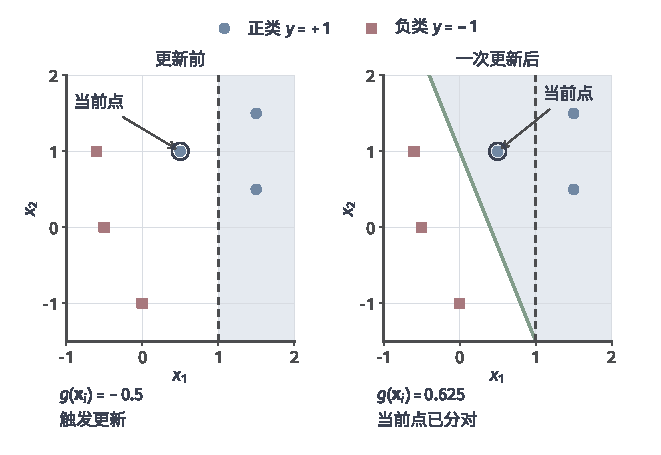
\includegraphics[width=112.000mm]{figures/04-classic-models/00-shared/matplotlib/classification-perceptron-update/figure.pdf}
  \caption{错分正类点触发的一次感知机更新。六个点为教学构造，坐标无量纲，两面板共用坐标范围；蓝圆、红方分别为正负类，黑色圆环标出当前点。浅蓝区域为正类预测区域，虚线为旧边界$x_1=1$，绿色实线为新边界$1.25x_1+0.5x_2=0.5$。偏置随权重一起更新，当前点由负得分变为正得分。}
  \label{fig:classification-perceptron-update}
\end{figure}

\begin{algorithm}[带遍历上限的感知机训练]
  \label{alg:classification-perceptron}
  \begin{algorithmic}[1]
    \Require $D_n$，固定学习率$\eta>0$，最大遍历轮数$E\geq1$
    \Ensure 参数$\tilde{\bm{w}}$与是否已验证收敛的状态
    \State $\tilde{\bm{w}}\gets\bm{0}$
    \For{$e=1,\ldots,E$}
      \State $m\gets0$
      \For{$i=1,\ldots,n$}
        \State $\tilde{\bm{x}}_i\gets(\bm{x}_i^{\top},1)^{\top}$
        \If{$y_i\langle\tilde{\bm{w}},\tilde{\bm{x}}_i\rangle\leq0$}
          \State $\tilde{\bm{w}}\gets\tilde{\bm{w}}+\eta y_i\tilde{\bm{x}}_i$
          \State $m\gets m+1$
        \EndIf
      \EndFor
      \If{$m=0$}
        \State \Return $(\tilde{\bm{w}},\text{已收敛})$
      \EndIf
    \EndFor
    \State \Return $(\tilde{\bm{w}},\text{达到轮数上限})$
  \end{algorithmic}
\end{algorithm}

一整轮没有更新时，所有样本都是在同一个参数下得到严格正的有符号得分，才构成收敛证据。达到轮数上限时返回的是预算内的当前解，可分性仍未由这一停止状态判定。稠密实现每轮需要$O(nd)$运算，除训练集外只需$O(d)$参数空间；样本访问顺序可以改变输出的分隔面。

从优化角度看，定义\term{感知机损失}（perceptron loss）
\begin{equation}
  \label{eq:classification-perceptron-loss}
  \ell_{\mathrm{P}}(\tilde{\bm{w}};\bm{x}_i,y_i)
    =\max\{0,-y_i\langle\tilde{\bm{w}},\tilde{\bm{x}}_i\rangle\}.
\end{equation}
为了把这项损失用于更新，先看它的两段：当带符号得分为负时，对参数求导得到$-y_i\tilde{\bm{x}}_i$；得分为正时，损失恒为零，梯度也是$\bm 0$。两段在零得分处相接，却给出不同斜率，普通梯度在这里没有定义。由于损失仍是凸的，可以使用次梯度；在交点处选择$-y_i\tilde{\bm{x}}_i$，仍满足支撑损失的仿射下界条件，也就得到式~\eqref{eq:classification-perceptron-update}。这一求解依据见\BookSectionRef{sec:opt-subgradient-methods}{第一卷“数学准备”的“基于次梯度的求解”节}。

上述更新逐样本执行；随机抽取样本时才相应成为随机次梯度下降。这里使用的是零间隔损失，不是标准的\term{合页损失}（hinge loss）$\max\{0,1-y_i\langle\tilde{\bm{w}},\tilde{\bm{x}}_i\rangle\}$。前者在零参数处就对所有样本取零，因此“感知机损失为零”本身不能证明分类正确；算法在零得分处仍更新的约定不可省略。

\subsubsection{理论分析}
\label{sec:classification-perceptron-analysis}

\paragraph{表达能力}
单层感知机的候选规则为$\operatorname{sign}(\bm w^\top\bm x+b)$。目标本来就是一个半空间时，这个候选类可以精确表示它；目标依赖特征交互时，则可能无法同时满足全部类别条件。

例如，取$(1,1)$、$(-1,-1)$、$(1,-1)$、$(-1,1)$四点作为输入域，同号坐标的目标标签为$-1$，异号坐标为$+1$。正、负两对点的中点都在原点。若一个仿射得分把四点全分对，正类得分的平均必须非负，负类得分的平均必须为负；两者却都等于$b$，产生矛盾。因此候选类中的每个函数至少在一个点上偏离目标。增加特征$x_1x_2$后，得分$-x_1x_2$恰好满足四点的目标标签，这才改变了候选空间的表示限制。

\paragraph{收敛性}
每次修正可能破坏已有判断，为什么这些修正不会无穷持续？关键是存在一个始终把所有样本分对的参考方向：更新朝该方向取得线性累积的进展，而参数范数的平方只能线性增长。Novikoff在1962年报告的证明清楚展示了这两个增长速度之间的矛盾\scite{novikoff1962}。

\begin{theorem}[感知机在有界可分样本下的最大更新次数]
  \label{thm:classification-perceptron-mistakes}
  若$D_n$满足式~\eqref{eq:classification-perceptron-margin}，从零参数出发，以固定$\eta>0$按式~\eqref{eq:classification-perceptron-update}更新，则对任意样本访问顺序，错误更新次数$M$满足
  \[
    M\leq\left(\frac R\gamma\right)^2 .
  \]
  这里错误更新包括零得分时的更新。若持续完整遍历训练集，且不因预算提前退出，算法在有限轮后得到所有训练样本上有符号得分均严格为正的参数。
\end{theorem}

\begin{proof}
  设第$t+1$次更新使用样本$i_t$。沿单位参考方向$\bm{u}^\ast$考察更新，得到
  \begin{align*}
    \langle\tilde{\bm{w}}^{(t+1)},\bm{u}^\ast\rangle
      &=\langle\tilde{\bm{w}}^{(t)},\bm{u}^\ast\rangle
        +\eta y_{i_t}\langle\tilde{\bm{x}}_{i_t},\bm{u}^\ast\rangle\\
      &\geq\langle\tilde{\bm{w}}^{(t)},\bm{u}^\ast\rangle+\eta\gamma .
  \end{align*}
  从零参数累加$M$次，便有
  \[
    \langle\tilde{\bm{w}}^{(M)},\bm{u}^\ast\rangle
      \geq M\eta\gamma .
  \]
  另一方面，展开更新后的平方范数：
  \begin{align*}
    \|\tilde{\bm{w}}^{(t+1)}\|_2^2
      &=\|\tilde{\bm{w}}^{(t)}\|_2^2
        +2\eta y_{i_t}
          \langle\tilde{\bm{w}}^{(t)},\tilde{\bm{x}}_{i_t}\rangle\\
      &\quad+\eta^2\|\tilde{\bm{x}}_{i_t}\|_2^2\\
      &\leq\|\tilde{\bm{w}}^{(t)}\|_2^2+\eta^2R^2 .
  \end{align*}
  不等式使用了更新条件：交叉项非正；并使用同一增广空间中的长度界$R$。再次累加，得到$\|\tilde{\bm{w}}^{(M)}\|_2^2\leq M\eta^2R^2$。由Cauchy--Schwarz不等式和$\|\bm{u}^\ast\|_2=1$，
  \[
    M\eta\gamma
      \leq\langle\tilde{\bm{w}}^{(M)},\bm{u}^\ast\rangle
      \leq\|\tilde{\bm{w}}^{(M)}\|_2
      \leq\eta R\sqrt{M}.
  \]
  $M=0$时结论直接成立；$M>0$时除以$\eta\sqrt M$再平方，得到所述界。因此更新不可能无限发生。持续完整遍历会在最后一次更新之后再检查所有样本；若仍有非正得分就还会更新，产生矛盾，故最终必有一整轮没有更新。
\end{proof}

这个界不显式含$n$，也不依赖访问顺序，但$R$和$\gamma$随数据而定；增加样本可能缩小可分间隔。它只约束更新次数，不包括寻找错误时检查正确样本的开销。对于算法~\ref{alg:classification-perceptron}的逐轮扫描，若不提前截断，至多需要$M+1$轮，包括最终的无更新确认轮。

若数据不可分，有限更新保证失效，持续遍历可能反复更新，此时可以限制训练预算并保留历史较好解，或采用允许间隔违约的在线方法。这些处理改变了停止或选解方式，仍须分别分析。

\paragraph{泛化性}
测试风险需要训练更新之外的统计条件。前述错误次数证明只考察给定样本的几何结构；若要判断未来预测，需要规定抽样分布与训练后返回哪个分类器。Cesa-Bianchi、Conconi与Gentile在2004年研究了这种联系：由独立同分布样本上的在线表现控制历史预测规则的风险，并讨论相应的输出选择方法\scite{cesabianchi2004generalization}。

下面给出一个期望风险的简单结论，说明额外条件怎样进入证明。按独立同分布的到达顺序，仅遍历$D_n$一次，从零参数出发使用固定学习率$\eta>0$和原更新规则。用$f_i$表示看到第$i$个样本之前的分类器；它只依赖$D_{i-1}$，其中$D_0$为空。这里$i$计数已访问的样本位置，与只计实际更新的$t$不同。训练后独立地从$\{1,\ldots,n\}$均匀抽取$I$，返回$f_I$，使输出规则与下述期望风险证明一致。

\begin{theorem}[感知机随机历史输出在可分分布下的期望风险界]
  \label{thm:classification-perceptron-risk}
  设训练样本独立同分布，测试样本独立来自同一分布。假设存在固定的单位向量$\bm{u}^\ast$及常数$R<\infty$、$\gamma>0$，使
  \[
    \|\tilde{\bm{x}}\|_2\leq R,\qquad
    y\langle\bm{u}^\ast,\tilde{\bm{x}}\rangle\geq\gamma
    \quad\text{几乎必然}.
  \]
  对上述单遍历训练和随机输出规则，有
  \begin{equation}
    \label{eq:classification-perceptron-risk}
    \mathbb{E}_{D_n,I}\!\left[R(f_I\mid D_n,I)\right]
      \leq\frac{R^2}{n\gamma^2}.
  \end{equation}
\end{theorem}

\begin{proof}
  令$e_i=\mathbb{1}\{f_i(\bm{x}_i)\ne y_i\}$。由于$f_i$尚未使用第$i$个样本，独立性给出
  \[
    \mathbb{E}[e_i\mid D_{i-1}]
      =R(f_i\mid D_{i-1}).
  \]
  对两边取期望，再对均匀的$I$平均，就有
  \[
    \mathbb{E}_{D_n,I}[R(f_I\mid D_n,I)]
      =\frac1n\sum_{i=1}^{n}\mathbb{E}[e_i].
  \]
  每次预测错误都会触发更新，零得分且预测正确时也可能更新，故$\sum_i e_i\leq M$。分布层面的共同间隔和长度界使定理~\ref{thm:classification-perceptron-mistakes}几乎必然适用于每个训练序列，于是$M\leq R^2/\gamma^2$，代入即得结论。
\end{proof}

这里的$R$和$\gamma$约束整个数据分布。式~\eqref{eq:classification-perceptron-risk}对训练抽样及随机历史状态取平均；当上界小于$1$时，它提供非平凡的期望风险控制。最终参数或多轮训练使用不同的输出与依赖关系，需各自分析：尤其在多轮中，当前样本已经参与既有参数的形成。不同的历史选解规则需要分别检查其训练依赖。

\subsubsection{优化表达能力}

若问题在于原空间不能线性分开，可把输入换成特征映射$\bm{\phi}(\bm{x})$。核函数$K(\bm{x},\bm{z})=\langle\bm{\phi}(\bm{x}),\bm{\phi}(\bm{z})\rangle$直接计算映射后的内积，省去显式构造高维坐标，得到\term{核感知机}（kernel perceptron）。为与前文偏置一致，使用增广映射$(\bm{\phi}(\bm{x}),1)$及其核$\tilde K(\bm{x},\bm{z})=K(\bm{x},\bm{z})+1$。零初始化、单位学习率下，参数在特征空间中是更新样本的线性组合，预测可写为
\begin{equation}
  \label{eq:classification-kernel-perceptron}
  f(\bm{x})=\operatorname{sign}
    \left(\sum_{i=1}^{n}\alpha_i y_i
      [K(\bm{x}_i,\bm{x})+1]\right).
\end{equation}
这里$\alpha_i$是样本$i$的更新次数；遇到非正有符号得分时令$\alpha_i\leftarrow\alpha_i+1$。必须选用正定核，即它在任意有限输入集上生成半正定Gram矩阵，才能作上述内积解释；有限更新还要求增广特征空间内存在正间隔，长度界相应变为$\sqrt{K(\bm{x}_i,\bm{x}_i)+1}$的上界。预测需要访问系数非零的样本，数量可能随训练增长。将内积推广到特征空间的思路可追溯至Aizerman、Braverman与Rozonoer在1964年的势函数研究\scite{aizerman1964}。

核与输入尺度共同决定映射后是否可分；预测成本则由需要保存的更新样本数决定。核化改变表示，不替代对标签噪声、停止规则和样本外误差的检查。

\subsubsection{优化泛化能力}

若希望减轻预测对最后一次参数更新的依赖，可以汇总训练过程中的多个状态。Freund与Schapire在1999年研究的\term{投票感知机}（voted perceptron）保存历次权重，并按各状态持续使用的次数加权投票；同一论文也比较了用历史得分平均代替投票的方式\scite{freund1999}。沿用本节的增广表示，设保存的状态为$\tilde{\bm w}_1,\ldots,\tilde{\bm w}_K$，$c_k>0$是第$k$个状态的计数，则投票预测为
\begin{equation}
  f_{\mathrm V}(\bm x)
  =\operatorname{sign}\!\left[
    \sum_{k=1}^{K}c_k\operatorname{sign}
       (\tilde{\bm w}_k^\top\tilde{\bm x})\right].
  \label{eq:classification-voted-perceptron}
\end{equation}
计数必须与更新同步。初始零参数的计数取零；本次检查未触发更新时，将当前状态的计数加一；触发更新时，保存新参数并把新状态的计数置为一，不再给被替换的旧状态加一。这里沿用非正有符号得分触发更新的约定，最后忽略计数为零的状态。计数取决于访问顺序与训练预算，并不是对新样本准确率的独立测量。保存与预测$K$个稠密状态均需考虑$O(Kd)$的代价。

\term{平均感知机}（averaged perceptron）改为先把这些增广参数平均：
\[
  \bar{\bm w}=\frac{\sum_{k=1}^{K}c_k\tilde{\bm w}_k}
                        {\sum_{k=1}^{K}c_k},
  \qquad
  f_{\mathrm A}(\bm x)=\operatorname{sign}
                    (\bar{\bm w}^\top\tilde{\bm x}).
\]
线性实现可在训练时累计参数和，最终只保存一组参数，额外存储与单次预测均为$O(d)$。投票先对每个得分取符号，再汇总标签；参数平均先汇总实值得分，再取符号，二者一般不同。前者的最终规则可以组合多个半空间判断，后者仍返回单个仿射得分；它们都改变训练结束后的输出方式，不能仅凭“汇总历史”判断哪种更适合任务。

\subsubsection{优化计算能力}

\paragraph{保存预算内的较优参数}
不可分数据可能使参数反复改变，预算结束时的权重未必是已经检查过的最好结果。\term{口袋算法}（Pocket algorithm）通过保存历史参数处理这个问题。常用版本额外保存$\tilde{\bm{w}}_{\mathrm{pocket}}$：每次检查候选参数时，计算全训练集零一错误数，仅在严格改进时替换记录；预算用尽后返回记录参数。它适用于噪声或矛盾标签数据，返回预算内已检查候选中的最小训练错误解；每次候选比较还需要评估全训练集。Gallant在1990年的论文中系统讨论了Pocket及相关学习方法\scite{gallant1990}。

Pocket只改变返回哪组历史参数，候选得分仍是原坐标中的仿射函数。它需要额外评估全部训练样本，也不能消除前面异或任务的表示限制。这里改善的是有限预算下的返回规则，并未使不可分数据上的原更新停止，也不保证找到所有仿射分类器中的最小训练错误解。

\paragraph{控制单步参数改动}
若希望每次更新不仅改正符号，还达到指定得分间隔，\term{被动攻击算法}（passive-aggressive algorithm, PA）把“尽量少改参数”和“满足当前样本的单位间隔”合成一个投影问题。用$\bm{v}$表示待求的新增广参数，
\begin{equation}
  \label{eq:classification-pa-projection}
  \begin{aligned}
    \min_{\bm{v}}\quad&
      \frac12\|\bm{v}-\tilde{\bm{w}}\|_2^2\\
    \text{满足}\quad&
      y_i\langle\bm{v},\tilde{\bm{x}}_i\rangle\geq1 .
  \end{aligned}
\end{equation}
令$\ell_i=\max\{0,1-y_i\langle\tilde{\bm{w}},\tilde{\bm{x}}_i\rangle\}$。约束已满足时参数不变；否则，拉格朗日驻点要求$\bm{v}=\tilde{\bm{w}}+\tau_i y_i\tilde{\bm{x}}_i$，将活跃约束代回即得
\[
  \tau_i=\frac{\ell_i}{\|\tilde{\bm{x}}_i\|_2^2},
  \qquad
  \tilde{\bm{w}}\leftarrow
    \tilde{\bm{w}}+\tau_i y_i\tilde{\bm{x}}_i .
\]
因此PA在间隔足够时“被动”，不足时按违约大小调整。增广方式也意味着这里把偏置变化纳入距离惩罚。噪声下硬性满足当前样本可能调整过大，PA-I可用$\tau_i=\min\{\lambda_{\mathrm{PA}},\ell_i/\|\tilde{\bm{x}}_i\|_2^2\}$限制步长，其中$\lambda_{\mathrm{PA}}>0$控制容忍程度。Crammer等人的2006年论文统一分析了这些在线大间隔方法；其保证针对在线更新的损失与间隔行为\scite{crammer2006}。
PA的单位间隔要求改变单步参数选择，候选得分仍是仿射函数。因此它与基本感知机、Pocket共享原坐标中的表示限制；间隔要求本身不能表达异或交互。

\subsubsection{支持多分类预测场景}

\label{sec:classification-perceptron-multiclass}

对$C$类问题，把标签改为$y_i\in\{1,\ldots,C\}$，每类维护一组增广参数$\tilde{\bm{w}}_c=(\bm{w}_c^{\top},b_c)^{\top}$，得分和预测为
\[
  s_c(\bm{x})=\langle\tilde{\bm{w}}_c,\tilde{\bm{x}}\rangle,
  \qquad
  \hat y=\argmax_{c\in\{1,\ldots,C\}}s_c(\bm{x}).
\]
平局仍按最小类别索引处理。这个构造把正确类别的得分与每个竞争类别作比较，也可用\term{Kesler构造}（Kesler construction）把这些比较写成一个扩展空间中的线性可分问题。

第$c$类获胜要求$s_c(\bm x)\geq s_j(\bm x)$对每个竞争类成立，平局处再按既定顺序处理。因此每类区域是若干半空间的交，仍是凸区域。它可以表示多类线性分区，却不能在原坐标中把某一类分成被其他类别隔开的多个区域；这种任务需要新的特征或不同的输出表示。

遇到$\hat y_i\ne y_i$时，只提高正确类别的参数并降低错误获胜类别的参数：
\begin{equation}
  \label{eq:classification-perceptron-multiclass-update}
  \begin{aligned}
    \tilde{\bm{w}}_{y_i}
      &\leftarrow\tilde{\bm{w}}_{y_i}+\eta\tilde{\bm{x}}_i,\\
    \tilde{\bm{w}}_{\hat y_i}
      &\leftarrow\tilde{\bm{w}}_{\hat y_i}-\eta\tilde{\bm{x}}_i .
  \end{aligned}
\end{equation}
其余类别不变，两个类别的偏置也随各自最后一个分量同时更新。若平局后预测错误，同样更新；若已选择正确类别，则该规则不更新。与二分类中所有零得分均更新的约定不同，这里直接按最终预测是否正确判断。

收敛条件也必须改为多类的得分差条件。把各类参数按行堆成$\tilde{\bm{W}}\in\mathbb{R}^{C\times(d+1)}$；假设存在$\|\bm{U}^\ast\|_{\mathrm{F}}=1$和$\gamma_{\mathrm{mc}}>0$，使对所有$i$和$c\ne y_i$都有
\[
  \langle\bm{U}_{y_i,:}^\ast-\bm{U}_{c,:}^\ast,
    \tilde{\bm{x}}_i\rangle\geq\gamma_{\mathrm{mc}} .
\]
这里$\|\cdot\|_{\mathrm{F}}$是所有矩阵元素平方和的平方根，行向量的内积按对应坐标计算。一次更新的方向矩阵仅两行非零，分别为$\tilde{\bm{x}}_i^{\top}$与$-\tilde{\bm{x}}_i^{\top}$，其平方范数至多为$2R^2$。它与$\bm{U}^\ast$的内积至少为$\gamma_{\mathrm{mc}}$；与当前参数的内积则为$s_{y_i}(\bm{x}_i)-s_{\hat y_i}(\bm{x}_i)\leq0$。因此零初始化时完全沿用二分类证明，得到
\[
  M\eta\gamma_{\mathrm{mc}}
    \leq\|\tilde{\bm{W}}^{(M)}\|_{\mathrm{F}}
    \leq\eta R\sqrt{2M},
  \qquad
  M\leq\frac{2R^2}{\gamma_{\mathrm{mc}}^2}.
\]
有限更新保证因而保留下来，但它要求所有正确类与竞争类之间都具有共同的正间隔，而不是只检查任意一对类别。

\subsubsection{支持结构化输出预测场景}

如果任务是给一句话中的每个词标注词性，输出就从一个类别变成了一整条标签序列。逐词独立判类无法在同一个得分中评价相邻标签的组合；我们希望同时比较不同候选序列，并在预测错误时调整整条序列用到的特征。\term{结构化感知机}（structured perceptron）把多分类的得分比较推广到结构之间，用联合特征$\bm{\phi}(\bm{x},y)$描述输入与候选结构，预测
\[
  \hat y_i=\argmax_{y\in Y(\bm{x}_i)}
    \langle\bm{\theta},\bm{\phi}(\bm{x}_i,y)\rangle ,
\]
其中$Y(\bm{x}_i)$是候选结构集合，$\bm{\theta}$是与联合特征同维的参数。解码错误时进行
\[
  \bm{\theta}\leftarrow\bm{\theta}
    +\eta\bigl[\bm{\phi}(\bm{x}_i,y_i)
      -\bm{\phi}(\bm{x}_i,\hat y_i)\bigr].
\]
联合特征决定哪些结构差异能够进入比较。若同一输入上的两个候选结构具有完全相同的$\bm\phi(\bm x,y)$，它们对所有参数都同分，候选得分无法区分两者，只能由固定的平局规则选择其中一个。词性标注中的相邻标签关系或更远处的依赖，因而需要由相应的特征记录；解码搜索再精确，也不能恢复特征没有保留的差异。

需要的类别或结构偏置也作为联合特征中的相应指示分量处理；对所有候选都相同的常数项会在得分差中消去。结构化输出增加了解码成本，近似解码还可能改变哪些样本触发更新，需要与特征设计一同评价。Collins在2002年将这种更新与参数平均用于序列标注，提供了词性标注和短语识别等实例，也为比较感知机与条件随机场等结构化模型提供了参照\scite{collins2002}。

\subsubsection{小结}
\label{sec:classification-perceptron-summary}

感知机用当前样本的标签直接修正边界，免去了先拟合类分布的步骤。一次更新提高当前样本的有符号得分，却可能改变其他样本的判断；因此样本顺序、停止预算和返回规则都属于实际学习过程。它提供简洁的增量训练方式，原坐标中的单个边界仍受仿射表示限制。

预算结束时怎样利用历史参数，是不可分或尚未收敛数据上的一个具体问题。Gallant讨论的Pocket保存已检查的较好状态，代价是重复评估训练集；Freund与Schapire的投票感知机让多个状态共同判类，代价是状态存储与多次预测。平均感知机把历史压缩成一组参数，减轻线性预测的负担，但它与标签投票采用不同的汇总规则。选择时需要比较同一访问顺序与预算下的分类误差和存储成本。

若缺的是非线性输入关系，核感知机把内积换到特征空间，预测则需要保留更新样本。PA处理的困难不同：当一步更新还不足以达到所需间隔时，Crammer等用最小参数改动满足当前约束，噪声下再限制过大的调整。它改变单步目标，原坐标中的表示仍然线性。

序列标注等结构化任务又需要改变输出比较。Collins的结构化感知机通过联合特征评价完整序列，解码成本随候选结构增加。输入表示、单步目标与输出结构解决不同困难，不能用增加遍历次数代替这些改变。
